\documentclass{article}
\usepackage{v-test-paper}
\usepackage{comment}
\usepackage{enumitem}
\renewcommand{\frac}[2]{\dfrac{#1}{#2}}


%\renewcommand{\ans}{\quad}
%\def\ansint#1{\quad}

\newenvironment{solution}{\par\noindent\color{red!85!black}$\Rightarrow$\vspace{0em}}{}
% \excludecomment{solution}
% \renewenvironment{solution}{}{}


\title{\textsc{Projectile Motion}}
\date{}
\begin{document}
\maketitle

\begin{center}
    \textsc{\textbf{Introductory Exercise 7.1}}
\end{center}

\begin{enumerate}
    \item Two particles are projected from a tower horizontally in opposite directions with velocities 10 m/s and 20 m/s. Find the time when their velocity vectors are mutually perpendicular. Take \( g = 10 \text{m/s}^2 \).
        \begin{solution}
            \begin{align*}
                \intertext{Momentum of the ball will change only along the normal($x$ direction).}
                \vec{J} &= \vec{p}_f-\vec{p}_i\\
                &= m\vec{v}_f-m\vec{v}_i\\
                &= m\left(\dfrac{3}{4}v_0\hat{i}\right)-m\left(v_0\hat{i}\right)\\
                &= -\dfrac{1}{4}mv_0\hat{i}\\
                &= -\dfrac{5}{4}mv_0\hat{i}
            \end{align*}
        \end{solution}
    \item Projectile motion is a 3-dimensional motion. Is this statement true or false?
    \item Projectile motion (at low speed) is uniformly accelerated motion. Is this statement true or false?
    \item A particle is projected from ground with velocity 50 m/s at 37\(^{\circ}\) from horizontal. Find velocity and displacement after 2 s. \( \sin 37^{\circ} = \frac{3}{5} \)
    \item A particle is projected from a tower of height 25 m with velocity 20\(\sqrt{2}\) m/s at 45\(^{\circ}\) Find the time when particle strikes with ground. The horizontal distance from the foot of tower where it strikes. Also find the velocity at the time of collision.
\end{enumerate}
    \begin{center}
        \textsc{\textbf{Introductory Exercise 7.2}}
    \end{center}

\begin{enumerate}
    \item A particle is projected from ground with velocity 40\(\sqrt{2}\) m/s at 45\(^{\circ}\) Find
    \begin{enumerate}
        \item velocity and
        \item displacement of the particle after 2 s. (\( g = 10 \text{m/s}^2 \))
    \end{enumerate}
    \item Under what conditions the formulae of range, time of flight and maximum height can be applied directly in case of a projectile motion?
    \item What is the average velocity of a particle projected from the ground with speed \( u \) at an angle \( \alpha \) with the horizontal over a time interval from beginning till it strikes the ground again?
    \item What is the change in velocity in the above question?
    \item A particle is projected from ground with initial velocity \( u = 20\sqrt{2} \text{m/s} \) at \( \theta = 45^{\circ} \). Find
    \begin{enumerate}
        \item \( R \), \( H \) and \( T \),
        \item velocity of particle after 1 s
        \item velocity of particle at the time of collision with the ground (x-axis).
    \end{enumerate}
    \item A particle is projected from ground at angle 45\(^{\circ}\) with initial velocity 20\(\sqrt{2}\) m/s. Find
    \begin{enumerate}
        \item change in velocity,
        \item magnitude of average velocity in a time interval from \( t = 0 \) to \( t = 3 \) s.
    \end{enumerate}
    \item The coach throws a baseball to a player with an initial speed of 20 m/s at an angle of 45\(^{\circ}\) with the horizontal. At the moment the ball is thrown, the player is 50 m from the coach. At what speed and in what direction must the player run to catch the ball at the same height at which it was released? (\( g = 10 \text{m/s}^2 \))
    \item A ball is thrown horizontally from a point 100 m above the ground with a speed of 20 m/s. Find (a) the time it takes to reach the ground, (b) the horizontal distance it travels before reaching the ground, (c) the velocity (direction and magnitude) with which it strikes the ground.
    \item A bullet fired at an angle of 30\(^{\circ}\)with the horizontal hits the ground 3.0 km away. By adjusting its angle of projection, can one hope to hit a target 5.0 away? Assume the muzzle speed to be fixed and neglect air resistance.
    \item A particle moves in the xy-plane with constant acceleration \( a \) directed along the negative y-axis. The equation of path of the particle has the form \( y = bx - cx^2 \), where \( b \) and \( c \) are positive constants. Find the velocity of the particle at the origin of coordinates.
\end{enumerate}

\pagebreak
    \begin{center}
        \textsc{\textbf{Introductory Exercise 7.3}}
    \end{center}
\begin{enumerate}
    \item Find time of flight and range of the projectile along the inclined plane as shown in figure.
    \begin{center}
        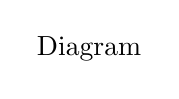
\begin{tikzpicture}
            \node {Diagram};
        \end{tikzpicture}
    \end{center}

    \item Find time of flight and range of the projectile along the inclined plane as shown in figure.
    \begin{center}
        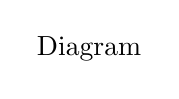
\begin{tikzpicture}
            \node {Diagram};
        \end{tikzpicture}
    \end{center}

    \item Find time of flight and range of the projectile along the inclined plane as shown in figure.
    \begin{center}
        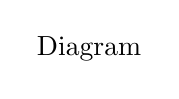
\begin{tikzpicture}
            \node {Diagram};
        \end{tikzpicture}
    \end{center}

    \item Passenger of a train just drops a stone from it. The train was moving with constant velocity. What is path of the stone as observed by (a) the passenger itself, (b) a man standing on ground?
    \item A particle is projected upwards with velocity 20 m/s. Simultaneously another particle is projected with velocity 20\(\sqrt{2}\) m/s at 45\(^{\circ}\). (\( g = 10 \text{m/s}^2 \))
    \begin{enumerate}
        \item What is acceleration of first particle relative to the second?
        \item What is initial velocity of first particle relative to the other?
        \item What is distance between two particles after 2 s?
    \end{enumerate}
    \item A particle is projected from the bottom of an inclined plane of inclination 30\(^{\circ}\). At what angle \( \alpha \) (from the horizontal) should the particle be projected to get the maximum range on the inclined plane.
\end{enumerate}

\pagebreak

\begin{center}
    \textsc{\textbf{Level I}}
\end{center}




\begin{center}
    \textsc{\textbf{Assertion and Reason}}
\end{center}

\begin{enumerate}[leftmargin=2cm]
    \item[1. Assertion:] A particle follows only a parabolic path if acceleration is constant.
    \item[Reason:] In projectile motion path is parabolic, as acceleration is assumed to be constant at low heights.
    
    \item[2. Assertion:] Projectile motion is called a two dimensional motion, although it takes place in space.
    \item[Reason:] In space it takes place in a plane.
    
    \item[3. Assertion:] If time of flight in a projectile motion is made two times, its maximum height will become four times.
    \item[Reason:] In projectile motion \( H \propto t^2 \), where \( H \) is maximum height and \( t \) the time of flight.
    
    \item[4. Assertion:] A particle is projected with velocity \( u \) at angle \( 45^\circ \) with ground. Let \( v \) be the velocity of particle at time \( t(> 0) \), then value of \( u \cdot v \) can be zero.
    \item[Reason:] Value of dot product is zero when angle between two vectors is \( 90^\circ \).
    
    \item[5. Assertion:] A particle has constant acceleration is \( x \)-\( y \) plane. But neither of its acceleration components (\( a_x \), and \( a_y \)) is zero. Under this condition particle cannot have parabolic path.
    \item[Reason:] In projectile motion, horizontal component of acceleration is zero.
    
    \item[6. Assertion:] In projectile motion at any two positions \( \frac{v_2 - v_1}{t_2 - t_1} \) always remains constant.
    \item[Reason:] The given quantity is average acceleration, which should remain constant as acceleration is constant.
    
    \item[7. Assertion:] Particle A is projected upwards. Simultaneously particle B is projected as projectile as shown. Particle A returns to ground in 4 s. At the same time particle B collides with A. Maximum height H attained by B would be 20 m. (\( g = 10 m s^{-2} \))
    \item[Reason:] Speed of projection of both the particles should be same under the given condition.
    
    \item[8. Assertion:] Two projectiles have maximum heights \( 4H \) and \( H \) respectively. The ratio of their horizontal components of velocities should be \( 1:2 \) for their horizontal ranges to be same.
    \item[Reason:] Horizontal range = horizontal component of velocity \( \times \) time of flight.
    
    \item[9. Assertion:] If \( g = 10 m/s^2 \) then in projectile motion speed of particle in every second will change by \( 10 ms^{-1} \).
    \item[Reason:] Acceleration is nothing but rate of change of velocity.
    
    \item[10. Assertion:] In projectile motion if particle is projected with speed \( u \), then speed of particle at height \( h \) would be \( \sqrt{u^2 - 2gh} \).
    \item[Reason:] If particle is projected with vertical component of velocity \( u_y \). Then vertical component at the height \( h \) would be \( \pm \sqrt{u_y^2 - 2gh} \)
\end{enumerate}

\begin{center}
    \textsc{\textbf{Objective Questions}}
\end{center}


\begin{enumerate}
    \item Identify the correct statement related to the projectile motion.
    \begin{tasks}(1)
        \task It is uniformly accelerated everywhere
        \task It is uniformly accelerated everywhere except at the highest position where it is moving with constant velocity
        \task Acceleration is never perpendicular to velocity
        \task None of the above
    \end{tasks}

    \item Two bodies are thrown with the same initial velocity at angles \(\theta\) and \(90^{\circ}-\theta\) respectively with the horizontal, their maximum heights are in the ratio
    \begin{tasks}(2)
        \task \(1 : 1\)
        \task \(\sin{\theta} : \cos{\theta}\)
        \task \(\sin^{2}{\theta} : \cos^{2}{\theta}\)
        \task \(\cos{\theta} : \sin{\theta}\)
    \end{tasks}

    \item The range of a projectile at an angle \(\theta\) is equal to half of the maximum range if thrown at the same speed. The angle of projection is given by
    \begin{tasks}(2)
        \task \(15^{\circ}\)
        \task \(30^{\circ}\)
        \task \(60^{\circ}\)
        \task data insufficient
    \end{tasks}

    \item A ball is projected with a velocity \(20 \text{ ms}^{-1}\) at an angle to the horizontal. In order to have the maximum range. Its velocity at the highest position must be
    \begin{tasks}(2)
        \task \(10 \text{ ms}^{-1}\)
        \task \(14 \text{ ms}^{-1}\)
        \task \(18 \text{ ms}^{-1}\)
        \task \(16 \text{ ms}^{-1}\)
    \end{tasks}

    \item The particle has initial velocity, \(v = 3\hat{i} + 4\hat{j}\) and a constant force \(F = 4\hat{i} - 3\hat{j}\) acts on it. The path of the particle is
    \begin{tasks}(2)
        \task straight line
        \task parabolic
        \task circular
        \task elliptical
    \end{tasks}

    \item A body is projected at an angle \(60^{\circ}\) with the horizontal with kinetic energy \(K\). When the velocity makes an angle \(30^{\circ}\) with the horizontal, the kinetic energy of the body will be
    \begin{tasks}(2)
        \task \(K/2\)
        \task \(K/3\)
        \task \(2K/3\)
        \task \(3K/4\)
    \end{tasks}

    \item If \(T_1\) and \(T_2\) are the times of flight for two complementary angles, then the range of projectile \(R\) is given by
    \begin{tasks}(2)
        \task \(R = 4gT_1T_2\)
        \task \(R = 2gT_1T_2\)
        \task \(R = \frac{1}{4}gT_1T_2\)
        \task \(R = \frac{1}{2}gT_1T_2\)
    \end{tasks}

    \item A gun is firing bullets with velocity \(v_0\) by rotating it through \(360^{\circ}\) in the horizontal plane. The maximum area covered by the bullets is
    \begin{tasks}(2)
        \task \(\frac{2}{3}\frac{\pi v_0^4}{g}\)
        \task \(\frac{\pi v_0^2}{g}\)
        \task \(\frac{1}{2}\frac{\pi v_0^4}{g^2}\)
        \task \(\frac{\pi v_0^4}{g}\)
    \end{tasks}

    \item A grass hopper can jump maximum distance 1.6 m. It spends negligible time on ground. How far can it go in \(10\sqrt{2} s\) ?
    \begin{tasks}(2)
        \task \(45 m\)
        \task \(30 m\)
        \task \(20 m\)
        \task \(40 m\)
    \end{tasks}

    \item Two stones are projected with the same speed but making different angles with the horizontal. Their horizontal ranges are equal. The angle of projection of one is \(\frac{\pi}{3}\) and the maximum height reached by it is \(102 m\). Then the maximum height reached by the other in metres is
    \begin{tasks}(2)
        \task \(76\)
        \task \(56\)
        \task \(34\)
        \task \(84\)
    \end{tasks}

    \item A ball is projected upwards from the top of a tower with a velocity \(50 ms^{-1}\) making an angle \(30^{\circ}\) with the horizontal. The height of tower is \(70 m\). After how many seconds from the instant of throwing, will the ball reach the ground. (\(g = 10 ms^{-2}\))
    \begin{tasks}(2)
        \task \(2 s\)
        \task \(5 s\)
        \task \(7 s\)
        \task \(9 s\)
    \end{tasks}

    \item Average velocity of a particle in projectile motion between its starting point and the highest point of its trajectory is (projection speed = \(u\), angle of projection from horizontal = \(\theta\))
    \begin{tasks}(2)
        \task \(u \cos{\theta}\)
        \task \(\frac{u}{2} \sqrt{1 + 3 \cos^2{\theta}}\)
        \task \(\frac{u}{2} \sqrt{2 + \cos^2{\theta}}\)
        \task \(\frac{u}{2} \sqrt{1 + \cos^2{\theta}}\)
    \end{tasks}

    \item A train is moving on a track at \(30 ms^{-1}\). A ball is thrown from it perpendicular to the direction of motion with \(30 ms^{-1}\) at \(45^{\circ}\) from horizontal. Find the distance of ball from the point of projection on train to the point where it strikes the ground.
    \begin{tasks}(2)
        \task \(90 m\)
        \task \(60 m\)
        \task \(60 m \sqrt{3}\)
        \task \(60 m \sqrt{3}\)
    \end{tasks}

    \item A body is projected at time \(t = 0\) from a certain point on a planet's surface with a certain velocity at a certain angle with the planet's surface (assumed horizontal). The horizontal and vertical displacements \(x\) and \(y\) (in metre) respectively vary with time \(t\) in second as, \(x = (10\sqrt{3}) t\) and \(y = 10t - t^{2}\). The maximum height attained by the body is
    \begin{tasks}(2)
        \task \(75 m\)
        \task \(100 m\)
        \task \(50 m\)
        \task \(25 m\)
    \end{tasks}

    \item A particle is fired horizontally from an inclined plane of inclination \(30^{\circ}\) with horizontal with speed \(50 ms^{-1}\). If \(g = 10 ms^{-2}\), the range measured along the incline is
    \begin{tasks}(2)
        \task \(500 m\)
        \task \(\frac{1000}{3} m\)
        \task \(200\sqrt{2} m\)
        \task \(100\sqrt{3} m\)
    \end{tasks}

    \item A fixed mortar fires a bomb at an angle of \(53^{\circ}\) above the horizontal with a muzzle velocity of \(80 ms^{-1}\). A tank is advancing directly towards the mortar on level ground at a constant speed of \(5 ms^{-1}\). The initial separation (at the instant mortar is fired) between the mortar and tank, so that the tank would be hit is [Take \(g = 10 ms^{-2}\)]
    \begin{tasks}(2)
        \task \(662.4 m\)
        \task \(626.3 m\)
        \task \(486.6 m\)
        \task \(506.6 m\)
    \end{tasks}
\end{enumerate}


\begin{center}
    \textsc{\textbf{Subjective Questions}}
\end{center}


\begin{enumerate}
    \item At time $t = 0$, a small ball is projected from point A with a velocity of 60 m/s at $60^\circ$ angle with horizontal. Neglect atmospheric resistance and determine the two times $t_1$ and $t_2$ when the velocity of the ball makes an angle of $45^\circ$ with the horizontal x-axis.
    \item A particle is projected from ground with velocity $20\sqrt{2}$ m/s at $45^\circ$. At what time particle is at height 15 m from ground? ($g = 10$ m/s$^2$)
    \item A particle is projected at an angle $60^\circ$ with horizontal with a speed $u = 20$ m/s. Taking $g = 10$ m/s$^2$. Find the time after which the speed of the particle remains half of its initial speed.
    \item Two particles A and B are projected from ground towards each other with speeds 10 m/s and $5\sqrt{2}$ m/s at angles $30^\circ$ and $45^\circ$ with horizontal from two points separated by a distance of 15 m. Will they collide or not?
    \begin{center}
        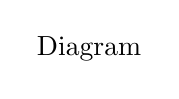
\begin{tikzpicture}
            \node {Diagram};
        \end{tikzpicture}
    \end{center}

    
    \item Two particles move in a uniform gravitational field with an acceleration $g$. At the initial moment the particles were located over a tower at one point and moved with velocities $v_1 = 3$ m/s and $v_2 = 4$ m/s horizontally in opposite directions. Find the distance between the particles at the moment when their velocity vectors become mutually perpendicular.
    
    \item A ball is thrown from the ground to clear a wall 3 m high at a distance of 6 m and falls 18 m away from the wall. Find the angle of projection of ball.

    \item A body is projected up such that its position vector varies with time as $r = \{3t i + (4t - 5t^2) j\}$ m. Here, t is in seconds. Find the time and x-coordinate of point when its y-coordinate is zero.

    \item A particle is projected along an inclined plane as shown in the figure. What is the speed of the particle when it collides at point A? ($g = 10$ m/s$^2$)
    \begin{center}
        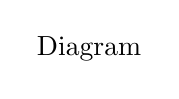
\begin{tikzpicture}
            \node {Diagram};
        \end{tikzpicture}
    \end{center}

    \item In the above problem, what is the component of its velocity perpendicular to the plane when it strikes at A?

    \item Two particles A and B are projected simultaneously from two towers of heights 10 m and 20 m respectively. Particle A is projected with an initial speed of $10\sqrt{2}$ m/s at an angle of $45^\circ$ with horizontal, while particle B is projected horizontally with speed 10 m/s. If they collide in air, what is the distance d between the towers?
    \begin{center}
        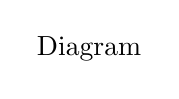
\begin{tikzpicture}
            \node {Diagram};
        \end{tikzpicture}
    \end{center}


    \item A particle is projected from the bottom of an inclined plane of inclination $30^\circ$ with velocity of 40 m/s at an angle of $60^\circ$ with horizontal. Find the speed of the particle when its velocity vector is parallel to the plane. Take $g = 10$ m/s$^2$.

    
    
    \item Two particles A and B are projected simultaneously in the directions shown in figure with velocities $u_A = 20$ m/s and $u_B = 10$ m/s respectively. They collide in air after $\frac{1}{2}$ s. Find \\
    (a) the angle $\theta$ \\
    (b) the distance x.
    \begin{center}
        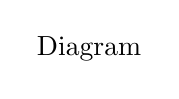
\begin{tikzpicture}
            \node {Diagram};
        \end{tikzpicture}
    \end{center}

    \item A ball is shot from the ground into the air. At a height of 9.1 m, its velocity is observed to be $v = 7.6\boldsymbol{\hat{i}} + 6.1\boldsymbol{\hat{j}}$ m/s (i is horizontal, j is upward). Give the approximate answers. \\
    (a) To what maximum height does the ball rise? \\
    (b) What total horizontal distance does the ball travel? \\
    (c) What are the magnitude and \\
    (d) What are the direction of the ball’s velocity just before it hits the ground?

    \item A particle is projected with velocity $2\sqrt{gh}$, so that it just clears two walls of equal height $h$ which are at a distance of $2h$ from each other. Show that the time of passing between the walls is $2\sqrt{\frac{2}{g}h}$.
    
    \item A particle is projected at an angle of elevation $\alpha$ and after $t$ seconds has to have elevation $\beta$ as seen from the point of projection. Find the initial velocity of projection.

    \item A projectile aimed at a mark, which is in the horizontal plane through the point of projection, falls a cm short of it when the elevation is $\alpha$ and goes b cm far when the elevation is $\beta$. Show that, if the speed of projection is same in all the cases the proper elevation is \\
    \[\frac{1}{2} \sin^{-1}\left[\frac{b \sin \alpha + a \sin \beta}{a + b}\right]\]

    \item Two particles are simultaneously thrown in horizontal direction from two points on a riverbank, which are at certain height above the water surface. The initial velocities of the particles are $u_1 = 5$ m/s and $u_2 = 7.5$ m/s respectively. Both particles fall into the water at the same time. First particle enters the water at a point s = 10 m from the bank. Determine \\
    (a) the time of flight of the two particles, \\
    (b) the height from which they are thrown, \\
    (c) the point where the second particle falls in water.
    \item A balloon is ascending at the rate $u = 12$ km/h and is being carried horizontally by the wind at $u_w = 20$ km/h. If a ballast bag is dropped from the balloon at the instant $h = 50$ m, determine the time needed for it to strike the ground. Assume that the bag was released from the balloon with the same velocity as the balloon. Also, find the speed with which the bag strikes the ground?

    \item A projectile is fired with a velocity $u$ at right angles to the slope, which is inclined at an angle $\theta$ with the horizontal. Derive an expression for the distance $R$ to the point of impact.
    \begin{center}
        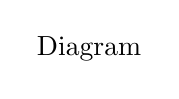
\begin{tikzpicture}
            \node {Diagram};
        \end{tikzpicture}
    \end{center}
    \item An elevator is going up with an upward acceleration of $1~\text{m/s}^2$. At the instant when its velocity is $2~\text{m/s}$, a stone is projected upward from its floor with a speed of $2~\text{m/s}$ relative to
the elevator, at an elevation of $30^\circ$.
    \begin{enumerate}
        \item Calculate the time taken by the stone to return to the floor.
        \item Sketch the path of the projectile as observed by an observer outside the elevator.
        \item If the elevator was moving with a downward acceleration equal to $g$, how would the motion be altered?
    \end{enumerate}
    \item Two particles $A$ and $B$ are projected simultaneously in a vertical plane as shown in figure. They collide at time $t$ in air. Write down two necessary equations for collision to take place.
    \begin{center}
        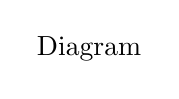
\begin{tikzpicture}
            \node {Diagram};
        \end{tikzpicture}
    \end{center}
\end{enumerate}

\begin{center}
    \textsc{\textbf{Level II}}
\end{center}


\begin{center}
    \textsc{\textbf{Multiple Choice Questions}}
\end{center}

\begin{enumerate}
    % Question 1
    \item Two bodies were thrown simultaneously from the same point, one straight up, and the other, at an angle of \(\theta = 30^{\circ}\) to the horizontal. The initial velocity of each body is \(20 \ ms^{-1}\). Neglecting air resistance, the distance between the bodies at \(t = 1.2\) later is
    \begin{tasks}(2)
        \task \(20 \ m\)
        \task \(30 \ m\)
        \task \(24 \ m\)
        \task \(50 \ m\)
    \end{tasks}
    % Question 2
    \item A particle is dropped from a height \(h\). Another particle which is initially at a horizontal distance \(d\) from the first is simultaneously projected with a horizontal velocity \(u\) and the two particles just collide on the ground. Then
    \begin{tasks}(2)
        \task \(d^2 = \frac{u^2 h}{2h}\)
        \task \(d^2 = \frac{2u^2 h}{g}\)
        \task \(d = h\)
        \task \(gd^2 = u^2 h\)
    \end{tasks}
    % Question 3
    \item A ball is projected from point A with velocity \(10 \ ms^{-1}\) perpendicular to the inclined plane as shown in figure. Range of the ball on the inclined plane is
    \begin{tasks}(4)
        \task \(\frac{40}{3} \ m\)
        \task \(\frac{20}{3} \ m\)
        \task \(\frac{12}{3} \ m\)
        \task \(\frac{60}{3} \ m\)
    \end{tasks}
    % Question 4
    \item A heavy particle is projected with a velocity at an angle with the horizontal into the uniform gravitational field. The slope of the trajectory of the particle varies as
    % Diagram for Question 4
    \begin{center}
        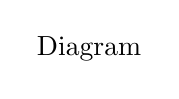
\begin{tikzpicture}
            \node {Diagram};
        \end{tikzpicture}
    \end{center}
    % Question 5
    \item A particle starts from the origin of coordinates at time \(t = 0\) and moves in the \(xy\) plane with a constant acceleration \(\alpha\) in the \(y\)-direction. Its equation of motion is \(y = \beta x^2\). Its velocity component in the \(x\)-direction is
    \begin{tasks}(2)
        \task \(\frac{2 \alpha}{\beta} \)
        \task \( \frac{\alpha}{\sqrt{\beta}} \)
        \task \( \frac{\alpha}{2 \beta} \)
        \task \( \frac{\alpha}{\sqrt{2\beta}} \)
    \end{tasks}
    % Question 6
    \item A projectile is projected with speed \(u\) at an angle of \(60^{\circ}\) with horizontal from an inclined plane. If the projectile hits the inclined plane horizontally, the range on inclined plane will be
    \begin{tasks}(2)
        \task \(\frac{u^2}{2\sqrt{2}g} \)
        \task \(\frac{3u^2}{2g} \)
        \task \(\frac{u^2}{\sqrt{2}g} \)
        \task \( \frac{\sqrt{2}u^2}{g} \)
    \end{tasks}
    % Question 7
    \item A particle is projected at an angle \(60^{\circ}\) with speed \(10 \sqrt{3} ms^{-1}\), from the point A, as shown in the figure. At the same time the wedge is made to move with speed \(10 \sqrt{3} ms^{-1}\) towards right as shown in the figure. Then the time after which particle will strike with wedge is
    \begin{tasks}(2)
        \task \(2s\)
        \task \(2\sqrt{3}s\)
        \task \(\frac{4}{\sqrt{3}}s\)
        \task None of these
    \end{tasks}
    % Question 8
    \item A particle moves along the parabolic path \(x - y^2 + 2y + 2\) in such a way that Y-component of velocity vector remains \(5 ms^{-1}\) during the motion. The magnitude of the acceleration of the particle is
    \begin{tasks}(2)
        \task \(50 ms^{-2}\)
        \task \(10 ms^{-2}\)
        \task \(10 \sqrt{2} ms^{-2}\)
        \task \(0.1 ms^{-2}\)
    \end{tasks}
    % Question 9
    \item A shell fired from the base of a mountain just clears it. If \(\alpha\) is the angle of projection, then the angular elevation of the summit \(\beta\) is
    \begin{center}
        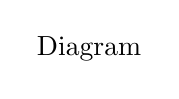
\begin{tikzpicture}
            \node {Diagram};
        \end{tikzpicture}
    \end{center}
    \begin{tasks}(2)
        \task \(\frac{\alpha}{2}\)
        \task \( \tan^{-1}\left(1\right) \)
        \task \( \tan^{-1}\left( \frac{\tan \alpha}{2} \right) \)
        \task \( \tan^{-1}\left( 2 \tan \alpha \right) \)
    \end{tasks}
    % Question 10
    \item In the figure shown, the two projectiles are fired simultaneously. The minimum distance between them during their flight is
    \begin{center}
        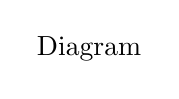
\begin{tikzpicture}
            \node {Diagram};
        \end{tikzpicture}
    \end{center}
    \begin{tasks}(2)
        \task \(20 m\)
        \task \(10 \sqrt{3} m\)
        \task \(10 m\)
        \task None of the above
    \end{tasks}
\end{enumerate}

\begin{center}
    \textsc{\textbf{More Than One Correct Options}}
\end{center}


\begin{enumerate}
    \item Two particles projected from the same point with same speed \( u \) at angles of projection \( \alpha \) and \( \beta \) strike the horizontal ground at the same point. If \( h_1 \) and \( h_2 \) are the maximum heights attained by the projectile, \( R \) is the range for both and \( t_1 \) and \( t_2 \) are their times of flights, respectively, then
    \begin{tasks}(2)
        \task \( \alpha + \beta = \frac{\pi}{2} \)
        \task \( R = 4 \sqrt{h_1 h_2} \)
        \task \( \frac{t_1}{t_2} = \tan \alpha \)
        \task \( \tan \alpha = \frac{h_1}{h_2} \)
    \end{tasks}
    
    \item A ball is dropped from a height of 49 m. The wind is blowing horizontally. Due to wind a constant horizontal acceleration is provided to the ball. Choose the correct statement (s).
    \begin{tasks}(2)
        \task Path of the ball is a straight line
        \task Path of the ball is a curved one
        \task The time taken by the ball to reach the ground is 3.16 s
        \task Actual distance traveled by the ball is more then 49 m
    \end{tasks}
    
    \item A particle is projected from a point \( P \) with a velocity \( u \) at an angle \( \theta \) with horizontal. At a certain point \( Q \) it moves at right angles to its initial direction. Then
    \begin{tasks}(2)
        \task velocity of particle at \( Q \) is \( u \sin \theta \)
        \task velocity of particle at \( Q \) is \( u \cos \theta \)
        \task time of flight from \( P \) to \( Q \) is \( (ug) \cos \theta \)
        \task time of flight from \( P \) to \( Q \) is \( (ulg) \sec \theta \)
    \end{tasks}
    
    \item At a height of 15 m from ground velocity of a projectile is \( \Vec{v} = (10\hat{i} + 10\hat{j}) \). Here, \( j \) is vertically upwards and \( i \) is along horizontal direction then
    \begin{tasks}(2)
        \task particle was projected at an angle of \( 45^{\circ} \) with horizontal
        \task time of flight of projectile is 4 s
        \task horizontal range of projectile is 100 m
        \task maximum height of projectile from ground is 20 m
    \end{tasks}
    
    \item Which of the following quantities remain constant during projectile motion?
    \begin{tasks}(2)
        \task Average velocity between two points
        \task \( \frac{dv}{dt} \)
        \task \( \frac{d^2v}{dt^2} \)
        \task Average speed between two points
    \end{tasks}
    
    \item In the projectile motion shown is figure, given \( t_{AB} = 2 \) s then
    \begin{center}
        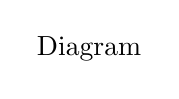
\begin{tikzpicture}
        \node {Diagram};
        \end{tikzpicture}
        \end{center}
    \begin{tasks}(2)
        \task particle is at point \( B \) at 3 s
        \task maximum height of projectile is 20 m
        \task initial vertical component of velocity is \( 20 \text{ ms}^{-1} \)
        \task horizontal component of velocity is \( 20 \text{ ms}^{-1} \)
    \end{tasks}
\end{enumerate}


\begin{center}
    \textsc{Comprehension-Based Questions}
\end{center}
Two inclined planes OA and OB intersect in a horizontal plane having their inclinations $\alpha$ and $\beta$ with the horizontal as shown in the figure. A particle is projected from point P with velocity $u$ along a direction perpendicular to plane OA. The particle strikes plane OB perpendicularly at Q.

\begin{center}
    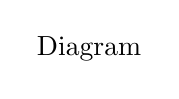
\begin{tikzpicture}
        \node at (0,0) {Diagram};
    \end{tikzpicture}
\end{center}

\begin{enumerate}
    \item If $\alpha = 30^\circ, \beta = 30^\circ$, the time of flight from P to Q is
    \begin{tasks}(4)
        \task $\frac{u}{g}$
        \task $\frac{\sqrt{3}u}{g}$
        \task $\frac{\sqrt{2}u}{g}$
        \task $\frac{2u}{g}$
    \end{tasks}
    
    \item If $\alpha = 30^\circ, \beta = 30^\circ$ and $a = 4.9$ m, the initial velocity of projection is
    \begin{tasks}(4)
        \task $9.8$ ms$^{-1}$
        \task $4.9$ ms$^{-1}$
        \task $4.9\sqrt{2}$ ms$^{-1}$
        \task $19.6$ ms$^{-1}$
    \end{tasks}
\end{enumerate}


\begin{center}
    \textsc{\textbf{Match The Columns}}
\end{center}


\begin{enumerate}
    \item Particle-1 is just dropped from a tower. 1 s later particle-2 is thrown from the same tower horizontally with velocity 10 ms$^{-1}$. Taking g = 10 m/s$^{2}$, match the following two columns at $t = 2$ s.
    \begin{center}
        \renewcommand{\arraystretch}{2}
        \begin{table}[h]
            \centering
            \begin{tabular}{p{0.25cm}p{8.5cm}|p{0.25cm}p{4.5cm}}
            \hline
            & Column I & & Column II \\
            \hline
            (a) & Horizontal displacement between two & (p) & 10 SI units \\
            (b) & Vertical displacement between two & (q) & 20 SI units \\
            (c) & Magnitude of relative horizontal component of velocity & (r) & 10$\sqrt{2}$ SI units \\
            (d) & Magnitude of relative vertical component of velocity & (s) & None of the above \\
            \hline
            \end{tabular}
        \end{table}
    \end{center}

    \item In a projectile motion, given $H = \frac{R}{2} = 20$ m. Here, $H$ is maximum height and $R$ the horizontal range. For the given condition match the following two columns.
    \begin{center}
        \renewcommand{\arraystretch}{2}
        \begin{table}[h]
            \centering
            \begin{tabular}{p{0.25cm}p{8.8cm}|p{0.25cm}p{4.5cm}}
            \hline
            & Column I & & Column II \\
            \hline
            (a) & Time of flight & (p) & 1 \\
            (b) & Ratio of vertical component of velocity and horizontal component of velocity & (q) & 2 \\
            (c) & Horizontal component of velocity (in m/s) & (r) & 10 \\
            (d) & Vertical component of velocity (in m/s) & (s) & None of the above \\
            \hline
            \end{tabular}
        \end{table}
    \end{center}

    \item A particle can be thrown at a constant speed at different angles. When it is thrown at 15$^{\circ}$ with horizontal, it falls at a distance of 10 m from point of projection. For this speed of particle match the following two columns.
    \begin{center}
        \renewcommand{\arraystretch}{2}
        \begin{table}[h]
            \centering
            \begin{tabular}{p{0.25cm}p{9.5cm}|p{0.25cm}p{3.5cm}}
            \hline
            & Column I & & Column II \\
            \hline
            (a) & Maximum horizontal range which can be taken with this speed & (p) & 10 m \\
            (b) & Maximum height which can be taken with this speed & (q) & 20 m \\
            (c) & Range at 75$^{\circ}$ & (r) & 15 m \\
            (d) & Height at 30$^{\circ}$ & (s) & None of the above \\
            \hline
            \end{tabular}
        \end{table}
    \end{center}

    \item In projectile motion, if vertical component of velocity is increased to two times, keeping horizontal component unchanged, then match the following two columns.
    \begin{center}
        \renewcommand{\arraystretch}{2}
        \begin{table}[h]
            \centering
            \begin{tabular}{p{0.25cm}p{8cm}|p{0.25cm}p{5cm}}
            \hline
            & Column I & & Column II \\
            \hline
            (a) & Time of flight & (p) & will remain same \\
            (b) & Maximum height & (q) & will become two times \\
            (c) & Horizontal range & (r) & will become four times \\
            (d) & Angle of projection with horizontal & (s) & None of the above \\
            \hline
            \end{tabular}
        \end{table}
    \end{center}

    \item In projectile motion shown in figure.
    \begin{center}
        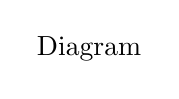
\begin{tikzpicture}
        \node {Diagram};
        \end{tikzpicture}
    \end{center}
    \begin{center}
        \renewcommand{\arraystretch}{2}
        \begin{table}[h]
            \centering
            \begin{tabular}{p{0.25cm}p{8cm}|p{0.25cm}p{5cm}}
            \hline
            & Column I & & Column II \\
            \hline
            (a) & Change in velocity between O and A & (p) & $u \cos \theta$ \\
            (b) & Change in velocity between A and B & (q) & $u \sin \theta$ \\
            (c) & Change in velocity between O and B & (r) & 2 $u \sin \theta$ \\
            (d) & Average velocity between O and B & (s) & None of the above \\
            \hline
            \end{tabular}
        \end{table}
    \end{center}

    \item Particle-1 is projected from ground (take it origin) at time $t = 0$, with velocity $(30\mathbf{i} + 30\mathbf{j})$ ms$^{-1}$. Particle-2 is projected from $(130 \text{m}, 75 \text{m})$ at time $t = 1$ s with velocity $(-20\mathbf{i} + 20\mathbf{j})$ ms$^{-1}$. Assuming $\mathbf{j}$ to be vertically upward and $\mathbf{i}$ to be in horizontal direction, match the following two columns at $t = 2$ s.
    \begin{center}
        \renewcommand{\arraystretch}{2}
        \begin{table}[h]
            \centering
            \begin{tabular}{p{0.25cm}p{8.5cm}|p{0.25cm}p{4.5cm}}
            \hline
            & Column I & & Column II \\
            \hline
            (a) & horizontal distance between two & (p) & 30 SI units \\
            (b) & vertical distance between two & (q) & 40 SI units \\
            (c) & relative horizontal component of velocity between two & (r) & 50 SI units \\
            (d) & relative vertical component of velocity between two & (s) & None of the above \\
            \hline
            \end{tabular}
        \end{table}
    \end{center}
    
    \item The trajectories of the motion of three particles are shown in the figure. Match the entries of Column I with the entries of Column II. Neglect air resistance.
    \begin{center}
        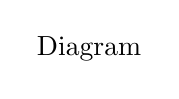
\begin{tikzpicture}
        \node {Diagram};
        \end{tikzpicture}
    \end{center}
    \begin{center}
        \renewcommand{\arraystretch}{2}
        \begin{table}[h]
            \centering
            \begin{tabular}{p{0.25cm}p{8cm}|p{0.25cm}p{5cm}}
            \hline
            & Column I & & Column II \\
            \hline
            (a) & Time of flight is least for & (p) & A \\
            (b) & Vertical component of velocity is greatest for & (q) & B \\
            (c) & Horizontal component of velocity is greatest for & (r) & C \\
            (d) & Launch speed is least for & (s) & same for all \\
            \hline
            \end{tabular}
        \end{table}
    \end{center}
\end{enumerate}

\pagebreak

\begin{center}
    \textsc{\textbf{Subjective Questions}}
\end{center}


\begin{enumerate}

    \item Determine the horizontal velocity \( v_0 \) with which a stone must be projected horizontally from a point \( P \), so that it may hit the inclined plane perpendicularly. The inclination of the plane with the horizontal is \( \theta \) and point \( P \) is at a height \( h \) above the foot of the incline, as shown in the figure.
    \begin{center}
    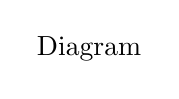
\begin{tikzpicture}
      \node {Diagram};
    \end{tikzpicture}
    \end{center}
  
    \item A particle is dropped from point \( P \) at time \( t = 0 \). At the same time another particle is thrown from point \( O \) as shown in the figure and it collides with the particle \( P \). Acceleration due to gravity is along the negative \( y \)-axis. If the two particles collide \( 2 \) s after they start, find the initial velocity \( v_0 \) of the particle which was projected from \( O \). Point \( O \) is not necessarily on ground.
    \begin{center}
    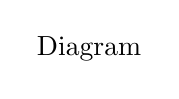
\begin{tikzpicture}
      \node {Diagram};
    \end{tikzpicture}
    \end{center}
  
    \item Two particles are simultaneously projected in the same vertical plane from the same point with velocities \( u \) and \( v \) at angles \( \alpha \) and \( \beta \) with horizontal. Find the time that elapses when their velocities are parallel.
    
    \item A projectile takes off with an initial velocity of \( 10 \) m/s at an angle of elevation of \( 45^\circ \). It is just able to clear two hurdles of height \( 2 \) m each, separated from each other by a distance \( d \). Calculate \( d \). At what distance from the point of projection is the first hurdle placed? Take \( g = 10 \) m/s\(^2\).
    
    \item A stone is projected from the ground in such a direction so as to hit a bird on the top of a telegraph post of height \( h \) and attains the maximum height of \( 2h \) above the ground. If at the instant of projection, the bird were to fly away horizontally with a uniform speed, find the ratio between the horizontal velocity of bird and the horizontal component of velocity of stone, if the stone hits the bird while descending.
  
    \item A particle is released from a certain height \( H = 400 \) m. Due to the wind, the particle gathers the horizontal velocity component \( v_x = at \) where \( a = 0.5 \) \( s^{-1} \) and \( y \) is the vertical displacement of the particle from the point of release, then find
    \begin{enumerate}
      \item the horizontal drift of the particle when it strikes the ground,
      \item the speed with which particle strikes the ground.
    \end{enumerate}
    (Take \( g = 10 \) m/s\(^2\))
  
    \item A train is moving with a constant speed of \( 10 \) m/s in a circle of radius \( \frac{16}{\pi} \) m. The plane of the circle lies in horizontal \( x \)-\( y \) plane. At time \( t = 0 \), train is at point \( P \) and moving in counter-clockwise direction. At this instant, a stone is thrown from the train with speed \( 10 \) m/s relative to train towards negative \( x \)-axis at an angle of \( 37^\circ \) with vertical \( z \)-axis. Find
    \begin{enumerate}
      \item the velocity of particle relative to train at the highest point of its trajectory.
      \item the coordinates of points on the ground where it finally falls and that of the highest point of its trajectory.
    \end{enumerate}
    (Take \( g = 10 \) m/s\(^2\), sin \( 37^\circ = \frac{3}{5} \), cos \( 37^\circ = \frac{4}{5} \))
  
    \item A particle is projected from an inclined plane \( OP_1 \) from \( A \) with velocity \( u_1 = 8 \) m/s\(^1 \) at angle \( 60^\circ \) with horizontal. An another particle is projected at the same instant from \( B \) vertically \( u_2 = 16 \) m/s\(^1 \) and perpendicular to the plane \( OP_1 \) from \( B \). After time \( t = 10\sqrt{3} \) s there separation was minimum and found to be \( 70 \) m. Then find distance \( AB \).
    \begin{center}
    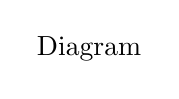
\begin{tikzpicture}
      \node {Diagram};
    \end{tikzpicture}
    \end{center}
  
    \item A particle is projected from point \( O \) on the ground with velocity \( \sqrt{5} \) m/s at angle \( \alpha = \tan^{-1}(0.5) \). It strikes at a point \( C \) on a fixed smooth plane \( AB \) having inclination of \( 37^\circ \) with horizontal as shown in figure. If the particle does not rebound, calculate
    \begin{enumerate}
      \item coordinates of point \( C \) in reference to coordinate system as shown in the figure.
      \item maximum height from the ground to which the particle rises.
    \end{enumerate}
    (Take \( g = 10 \) m/s\(^2\).)
  
    \item A plank fitted with a gun is moving on a horizontal surface with speed of \( 4 \) m/s along the positive \( x \)-axis. The \( z \)-axis is in vertically upward direction. The mass of the plank including the mass of the gun is \( 50 \) kg. When the plank reaches the origin, a shell of mass \( 10 \) kg is fired at an angle of \( 60^\circ \) with the positive \( x \)-axis with a speed of \( v = 20 \) m/s with respect to the gun in \( x \)-\( z \) plane. Find the position vector of the shell at \( t = 2 \) s after firing it. Take \( g = 9.8 \) m/s\(^2\).
  
  \end{enumerate}

  


  \begin{enumerate}
    \item Identify the correct statement related to the projectile motion.
        \begin{tasks}(1)
            \task It is uniformly accelerated everywhere
            \task It is uniformly accelerated everywhere except at the highest position where it is moving with constant velocity
            \task Acceleration is never perpendicular to velocity
            \task None of the above\ans
        \end{tasks}
    \begin{solution}
        Acceleration due to gravity is constant for a projectile throughout its motion, even at the topmost point of the trajectory where the velocity is momentarily horizontal.
        \begin{align*}
            \intertext{The correct answer is:}
            \text{(a) It is uniformly accelerated everywhere.}
        \end{align*}
    \end{solution}
    
    \item Two bodies are thrown with the same initial velocity at angles $\theta$ and $(90^\circ-\theta)$ respectively with the horizontal, their maximum heights are in the ratio
        \begin{tasks}(2)
            \task 1 : 1
            \task $\sin{\theta} : \cos{\theta}$
            \task $\sin^2{\theta} : \cos^2{\theta}$\ans
            \task $\cos{\theta} : \sin{\theta}$
        \end{tasks}
    \begin{solution}
        The maximum height is given by $h=\frac{u^2\sin^2{\theta}}{2g}$, and for complementary angles $\sin{\theta}=\cos{(90^\circ-\theta)}$. Thus, the ratio of maximum heights for $\theta$ and $90^\circ-\theta$ will be $\sin^2{\theta}:\cos^2{\theta}$.
    \end{solution}
    
    \item The range of a projectile at an angle $\theta$ is equal to half of the maximum range if thrown at the same speed. The angle of projection $\theta$ is given by
        \begin{tasks}(2)
            \task $15^\circ$
            \task $30^\circ$\ans
            \task $60^\circ$
            \task data insufficient
        \end{tasks}
    \begin{solution}
        Maximum range is achieved at $45^\circ$, so at angle $\theta$, the range $R=u^2\sin{2\theta}/g=u^2\sin{90^\circ}/2g$ (half of maximum range). Using $\sin{2\theta}=1/2$, we get $2\theta=30^\circ$, so $\theta=30^\circ$.
    \end{solution}
    
    \item A ball is projected with a velocity $20 ms^{-1}$ at an angle to the horizontal. In order to have the maximum range. Its velocity at the highest position must be
        \begin{tasks}(2)
            \task $10 ms^{-1}$
            \task $14 ms^{-1}$
            \task $18 ms^{-1}$
            \task $16 ms^{-1}$\ans
        \end{tasks}
    \begin{solution}
        For maximum range, the angle must be $45^\circ$, thus the horizontal component of velocity remains unchanged at the highest point. The initial horizontal velocity is thus $20\cos{45^\circ} = 20 \times \frac{\sqrt{2}}{2} ms^{-1}= 14 ms^{-1}$.
    \end{solution}
    
    \item A particle has initial velocity $\vec{v} = 3\hat{i} + 4\hat{j}$ and a constant force $\vec{F} = 4\hat{i} - 3\hat{j}$ acts on it. The path of the particle is
        \begin{tasks}(2)
            \task straight line
            \task parabolic\ans
            \task circular
            \task elliptical
        \end{tasks}
    \begin{solution}
        A constant force acting on a particle (neglecting gravity) would produce constant acceleration, thus causing the particle's path to be parabolic.
    \end{solution}
    
    \item A body is projected at an angle $60^\circ$ with the horizontal with kinetic energy $K$. When the velocity makes an angle $30^\circ$ with the horizontal, the kinetic energy of the body will be
        \begin{tasks}(2)
            \task $K/2$
            \task $K/3$
            \task $2K/3$\ans
            \task $3K/4$
        \end{tasks}
    \begin{solution}
        Kinetic energy is directly proportional to the square of the speed. At any point of the trajectory, the kinetic energy is the sum of the kinetic energies in the horizontal and vertical directions. Since horizontal kinetic energy remains constant, and vertical kinetic energy varies, we consider the vertical component at the $60^\circ$ and $30^\circ$ angles. Using trigonometry, we find the kinetic energy to be $2K/3$ when the angle is $30^\circ$.
    \end{solution}
    
    \item $T_1$ and $T_2$ are the times of flight for two complementary angles, then the range of projectile $R$ is given by
        \begin{tasks}(2)
            \task $R = 4gT_1T_2$
            \task $R = 2gT_1T_2$\ans
            \task $R = \frac{1}{4}gT_1T_2$
            \task $R = \frac{1}{2}gT_1T_2$
        \end{tasks}
    \begin{solution}
        The range $R$ for a projectile is given by $R=u^2\sin{2\theta}/g$. For complementary angles, the range is the same, so $R=u^2\sin{(\theta+(90^\circ-\theta))}/g=u^2/g$. The time of flights are $T_1$ and $T_2$, therefore $uT_1=gT_1/2$ and $uT_2=gT_2/2$, from which $R=2gT_1T_2$.
    \end{solution}
    
    \item A gun is firing bullets with velocity $v_0$ by rotating it through $360^\circ$ in the horizontal plane. The maximum area covered by the bullets is
        \begin{tasks}(2)
            \task $\frac{\pi v_0^4}{2g^2}$
            \task $\frac{\pi v_0^4}{g^2}$\ans
            \task $\frac{\pi v_0^4}{2g}$
            \task $\frac{\pi v_0^4}{g}$
        \end{tasks}
    \begin{solution}
        The maximum area would be a circle with the radius equal to the maximum range $R$. The range is given by $R = v_0^2/g$ for a projectile fired at $45^\circ$. Thus, the area $A = \pi R^2 = \pi (v_0^2/g)^2 = \pi v_0^4/g^2$.
    \end{solution}
    
    \item A grasshopper can jump maximum distance $1.6 m$. It spends negligible time on ground. How far can it go in $10\sqrt{2} s$ ?
        \begin{tasks}(2)
            \task $45 m$
            \task $30 m$
            \task $20 m$
            \task $40 m$\ans
        \end{tasks}
    \begin{solution}
        If the grasshopper jumps $1.6 m$ in each jump and spends negligible time on the ground, in $10\sqrt{2} s$ it would perform a number of jumps equal to $10\sqrt{2}/t_{jump}$, where $t_{jump}$ is the time for one jump. Assuming each jump takes the same time, the total distance is $1.6 m$ multiplied by the number of jumps. Without the time of a single jump, a specific solution is infeasible.
    \end{solution}
\end{enumerate}


\begin{enumerate}
    \item Identify the correct statement related to the projectile motion.
        \begin{tasks}(2)
            	\task It is uniformly accelerated everywhere
            	\task It is uniformly accelerated everywhere except at the highest position where it is moving with constant velocity
            	\task Acceleration is never perpendicular to velocity
            	\task None of the above
        \end{tasks}
    \begin{solution}
        \begin{align*}
            \intertext{The correct statement is that a projectile is uniformly accelerated everywhere due to the acceleration due to gravity, which acts downwards throughout the motion of the projectile.}
            \intertext{The correct option is:}
            \intertext{(a) It is uniformly accelerated everywhere}
        \end{align*}
    \end{solution}
    \item Two bodies are thrown with the same initial velocity at angles $\theta$ and $(90^\circ-\theta)$ respectively with the horizontal, then their maximum heights are in the ratio
        \begin{tasks}(2)
            	\task 1 : 1
            	\task $\sin{\theta} : \cos{\theta}$
            	\task $\sin^2{\theta} : \cos^2{\theta}$
            	\task $\cos{\theta} : \sin{\theta}$
        \end{tasks}
    % This is not a complete solution, it serves as an example.
    \begin{solution}
        \begin{align*}
            \intertext{Let $v$ be the initial velocity and $g$ be the acceleration due to gravity. The maximum height $h$ for a projectile launched at angle $\theta$ is given by $h = \frac{v^2 \sin^2{\theta}}{2g}$. Comparing the heights for angles $\theta$ and $(90^\circ-\theta)$, we get the ratio:}
            \frac{h_\theta}{h_{90^\circ-\theta}} &= \frac{\frac{v^2 \sin^2{\theta}}{2g}}{\frac{v^2 \cos^2{\theta}}{2g}} \\
            &= \frac{\sin^2{\theta}}{\cos^2{\theta}} \\
            &= \tan^2{\theta} \\
            \intertext{This can be rewritten in terms of sine and cosine to match the options.}
        \end{align*}
    \end{solution}
    % The remaining questions will be formatted without solutions for brevity.
    \item The range of a projectile at an angle $\theta$ is equal to half of the maximum range if thrown at the same speed. The angle of projection $\theta$ is given by
        \begin{tasks}(2)
            	\task $15^\circ$
            	\task $30^\circ$
            	\task $60^\circ$
            	\task data insufficient
        \end{tasks}
    \item A ball is projected with a velocity $20\ \mathrm{ms}^{-1}$ at an angle to the horizontal. In order to have the maximum range. Its velocity at the highest position must be
        \begin{tasks}(2)
            	\task $10\ \mathrm{ms}^{-1}$
            	\task $14\ \mathrm{ms}^{-1}$
            	\task $18\ \mathrm{ms}^{-1}$
            	\task $16\ \mathrm{ms}^{-1}$
        \end{tasks}
    \item The particle has initial velocity, $\vec{v} = 3\hat{i} + 4\hat{j}$ and a constant force $\vec{F} = 4\hat{i} - 3\hat{j}$ acts on it. The path of the particle is
        \begin{tasks}(2)
            	\task straight line
            	\task parabolic
            	\task circular
            	\task elliptical
        \end{tasks}
    \item A body is projected at an angle $60^\circ$ with the horizontal with kinetic energy $K$. When the velocity makes an angle $30^\circ$ with the horizontal, the kinetic energy of the body will be
        \begin{tasks}(2)
            	\task $K/2$
            	\task $K/3$
            	\task $2K/3$
            	\task $3K/4$
        \end{tasks}
    \item $T_1$ and $T_2$ are the times of flight for two complementary angles, then the range of projectile $R$ is given by
        \begin{tasks}(2)
            	\task $R = 4gT_1T_2$
            	\task $R = 2gT_1T_2$
            	\task $R = \frac{1}{4}gT_1T_2$
            	\task $R = \frac{1}{2}gT_1T_2$
        \end{tasks}
    \item A gun is firing bullets with velocity $v_0$ by rotating it through $360^\circ$ in the horizontal plane. The maximum area covered by the bullets is
        \begin{tasks}(2)
            	\task $\frac{\pi v_0^4}{2g^2}$
            	\task $\frac{\pi v_0^4}{g^2}$
            	\task $\frac{3\pi v_0^4}{2g^2}$
            	\task $\frac{\pi v_0^4}{8g^2}$
        \end{tasks}
    \item A grass hopper can jump maximum distance 1.6 m. It spends negligible time on ground. How far can it go in $10\sqrt{2}s$ ?
        \begin{tasks}(2)
            	\task $45\ m$
            	\task $30\ m$
            	\task $20\ m$
            	\task $40\ m$
        \end{tasks}
\end{enumerate}


\begin{enumerate}
    \item Identify the correct statement related to the projectile motion.
        \begin{tasks}(1)
            \task It is uniformly accelerated everywhere
            \task It is uniformly accelerated everywhere except at the highest position where it is moving with constant velocity
            \task Acceleration is never perpendicular to velocity
            \task None of the above \ans
        \end{tasks}
        
    \item Two bodies are thrown with the same initial velocity at angles \(\theta\) and \(90^\circ - \theta\) respectively with the horizontal, then their maximum heights are in the ratio
        \begin{tasks}(2)
            \task  \(1 : 1\) \ans
            \task  \(\sin \theta : \cos \theta\)
            \task  \(\sin^2 \theta : \cos^2 \theta\)
            \task  \(\cos \theta : \sin \theta\)
        \end{tasks}
    \begin{solution}
        \begin{align*}
            \intertext{The maximum height \(H\) reached by a projectile is given by \(H = \frac{u^2 \sin^2 \theta}{2g}\), where \(u\) is the initial velocity, \(g\) is the acceleration due to gravity, and \(\theta\) is the launch angle. For angles \(\theta\) and \(90^\circ - \theta\):}
            H_{\theta} &= \frac{u^2 \sin^2 \theta}{2g}, \\
            H_{90^\circ - \theta} &= \frac{u^2 \sin^2 (90^\circ - \theta)}{2g} = \frac{u^2 \cos^2 \theta}{2g}. \\
            \intertext{Taking the ratio of \(H_{\theta}\) to \(H_{90^\circ - \theta}\) gives:}
            \frac{H_{\theta}}{H_{90^\circ - \theta}} &= \frac{\sin^2 \theta}{\cos^2 \theta} = 1, \\
            \intertext{since \(\sin^2 \theta + \cos^2 \theta = 1\). Thus, the ratio is:}
            \frac{H_{\theta}}{H_{90^\circ - \theta}} &= 1.
        \end{align*}
    \end{solution}
    
    \item The range of a projectile at an angle \(\theta\) is equal to half of the maximum range if thrown at the same speed. The angle of projection \(\theta\) is given by
        \begin{tasks}(2)
            \task \(15^\circ\)
            \task \(30^\circ\) \ans
            \task \(60^\circ\)
            \task data insufficient
        \end{tasks}
    \begin{solution}
        \begin{align*}
            \intertext{The maximum range \(R_{\text{max}}\) for a given speed is obtained at an angle of \(45^\circ\). The range \(R\) at angle \(\theta\) is given by \(R = \frac{u^2 \sin 2\theta}{g}\). It is given that \(R = \frac{1}{2}R_{\text{max}}\), hence:}
            \frac{u^2 \sin 2\theta}{g} &= \frac{1}{2} \frac{u^2 \sin 90^\circ}{g}, \\
            \sin 2\theta &= \frac{1}{2}, \\
            2\theta &= 30^\circ \text{ or } 150^\circ, \\
            \intertext{Rejecting the obtuse angle as it is not relevant for the projectile motion, we have \(\theta\):}
            \theta &= 15^\circ.
        \end{align*}
    \end{solution}
    
    \item A ball is projected with a velocity 20 \(\text{ms}^{-1}\) at an angle to the horizontal. In order to have the maximum range. Its velocity at the highest position must be
        \begin{tasks}(2)
            \task \(10 \text{ms}^{-1}\)
            \task \(14 \text{ms}^{-1}\) \ans
            \task \(18 \text{ms}^{-1}\) 
            \task \(16 \text{ms}^{-1}\)
        \end{tasks}
    \begin{solution}
        \begin{align*}
            \intertext{The velocity at the highest point is horizontal and is equal to the initial horizontal component, which for a maximum range (launched at \(45^\circ\)) is:}
            v_{\text{horizontal}} &= u \cos 45^\circ = 20 \times \frac{1}{\sqrt{2}} \text{ms}^{-1}, \\
            &= 10\sqrt{2} \text{ms}^{-1} \approx 14 \text{ms}^{-1}.
        \end{align*}
    \end{solution}
        % Update this response once the image capability issue is resolved
    \item The particle has initial velocity, \(v = 3i + 4j\) and a constant force \(F = 4i - 3j\) acts on it. The path of the particle is
        \begin{tasks}(2)
            \task straight line
            \task parabolic \ans
            \task circular
            \task elliptical
        \end{tasks}
    \begin{solution}
        \begin{align*}
            \intertext{A constant force acting on a particle results in a constant acceleration. Thus, the motion of the particle is a form of uniformly accelerated motion, which results in a parabolic path.}
        \end{align*}
    \end{solution}
    
    \item A body is projected at an angle \(60^\circ\) with the horizontal with kinetic energy \(K\). When the velocity makes an angle \(30^\circ\) with the horizontal, the kinetic energy of the body will be
        \begin{tasks}(2)
            \task \(K/2\)
            \task \(K/3\) 
            \task \(2K/3\) \ans
            \task \(3K/4\)
        \end{tasks}
    \begin{solution}
        \begin{align*}
            \intertext{At the launch, the kinetic energy \(K\) is given by \(\frac{1}{2}mv^2\). When the velocity makes a \(30^\circ\) angle with the horizontal, the vertical component of the velocity reduces, and hence the total kinetic energy reduces. However, without specific values, we cannot calculate the exact proportion. If we assume no energy loss, the kinetic energy would be maximized at \(0^\circ\) and \(90^\circ\). Thus, if we have energy \(K\) at \(60^\circ\), it is hard to determine the precise energy at \(30^\circ\) without further information.}
            \intertext{However, typically, the kinetic energy would be a proportion of the original \(K\) corresponding to the decrease in the vertical component of the velocity.}
        \end{align*}
    \end{solution}
    
    \item \(T_1\) and \(T_2\) are the times of flight for two complementary angles, then the range of projectile \(R\) is given by
        \begin{tasks}(2)
            \task \(R = 4gT_1T_2\)
            \task \(R = 2gT_1T_2\)
            \task \(R = \frac{1}{4} gT_1T_2\) \ans
            \task \(R = \frac{1}{2} gT_1T_2\)
        \end{tasks}
    \begin{solution}
        \begin{align*}
            \intertext{The range \(R\) for a projectile is given by \(R = u^2 \frac{\sin 2\theta}{g}\) and the time of flight \(T\) is given by \(T = \frac{2u \sin \theta}{g}\). For complementary angles \(T_1\) and \(T_2\), we use \(\theta\) and \(90^\circ - \theta\). This gives \(T_1 = \frac{2u \sin \theta}{g}\) and \(T_2 = \frac{2u \cos \theta}{g}\), which leads to \(T_1T_2 = \frac{4u^2 \sin \theta \cos \theta}{g^2}\). Since \(\sin 2\theta = 2\sin \theta \cos \theta\), the range \(R\) is:}
            R &= u^2 \frac{2 \sin \theta \cos \theta}{g} \\
            &= g \frac{T_1T_2}{4}.
        \end{align*}
    \end{solution}
    
    \item A gun is firing bullets with velocity \(v_0\) by rotating it through \(360^\circ\) in the horizontal plane. The maximum area covered by the bullets is
        \begin{tasks}(2)
            \task \(\frac{\pi v_0^4}{2g^2}\)
            \task \(\frac{\pi v_0^4}{g^2}\) \ans
            \task \(\frac{\pi v_0^4}{3g^2}\)
            \task \(\frac{\pi v_0^4}{4g^2}\)
        \end{tasks}
    \begin{solution}
        \begin{align*}
            \intertext{When a gun fires bullets with velocity \(v_0\) at different angles, the maximum range is achieved at \(45^\circ\). The area covered is a circle with range \(R\) being the radius, so \(R = \frac{v_0^2}{g}\). The area \(A\) is:}
            A &= \pi R^2 = \pi \left(\frac{v_0^2}{g}\right)^2, \\
            &= \frac{\pi v_0^4}{g^2}.
        \end{align*}
    \end{solution}
    
    \item A grasshopper can jump maximum distance 1.6 m. It spends negligible time on ground. How far can it go in \(10\sqrt{2} s\) ?
        \begin{tasks}(2)
            \task 45 m 
            \task 30 m \ans
            \task 20 m 
            \task 40 m 
        \end{tasks}
    \begin{solution}
        \begin{align*}
            \intertext{If the grasshopper can jump a maximum distance of 1.6 m and spends negligible time on the ground, then in \(10\sqrt{2}\) seconds, the grasshopper would perform a series of jumps. The number of jumps \(n\) is given by dividing the total time by the time for each jump. Without the time for a single jump, we can't calculate the number of jumps. However, if a single jump takes \(t\) seconds, then:}
            n &= \frac{10\sqrt{2}}{t}, \\
            \intertext{And the total distance \(D\) would be:}
            D &= n \times 1.6 \, \text{m}.
        \end{align*}
    \end{solution}
\end{enumerate}


\begin{enumerate}
    \item Introductory Exercise 7.1
    \begin{enumerate}
      \item $\sqrt{2} s$
      \item False
      \item True
      \item $\mathbf{v} = (40i + 10j) \, \text{m/s}$, $\mathbf{s} = (80i + 40j) \, \text{m}$
      \item $t = 5 \, \text{s}, d = 100 \, \text{m}, \mathbf{v} = (20i - 30j) \, \text{ms}^{-1}$
    \end{enumerate}
  
    \item Introductory Exercise 7.2
    \begin{enumerate}
      \item (a) $20\sqrt{2} \, \text{m/s}$ at angle $\tan^{-1}\left(\frac{1}{2}\right)$ with horizontal, (b) 100 m.
      \item Between two points lying on the same horizontal line
      \item $v \cos \alpha$
      \item $v \sin \alpha$, downwards
      \item (a) $80 \, \text{m}, 20 \, \text{m}, 4 \, \text{s}$ (b) \[20i + 10j\] $\text{ms}^{-1}$ (c) \[20i - 20j\] $\text{ms}^{-1}$
      \item (a) $30 \, \text{ms}^{-1}$ (vertically downwards) (b) 20.62 $\text{ms}^{-1}$
      \item $\frac{5}{\sqrt{2}} \, \text{ms}^{-1}$
      \item (a) $\sqrt{20}$ (b) $20\sqrt{20} \, \text{m}$ (c) $49 \, \text{m/s}$, $\theta = \tan^{-1}(\sqrt{5})$ with horizontal
      \item No
      \item $\sqrt{\frac{a(1+b^{2})}{2c}}$
    \end{enumerate}
  
    \item Introductory Exercise 7.3
    \begin{enumerate}
      \item 1.69 s, 39 m
      \item 6.31 s, 145.71 m
      \item 2.31 s, 53.33 mm
      \item (a) A vertical straight line (b) A parabola
      \item (a) zero (b) 20 $\text{ms}^{-1}$ in horizontal direction (c) 40 m
      \item 60$^{\circ}Y$
    \end{enumerate}
  \end{enumerate}
  

\end{document}
